\documentclass[10pt,letterpaper]{article}
\usepackage[letterpaper, margin=1in]{geometry}
\usepackage[utf8]{inputenc}
\usepackage{amsmath}
\usepackage{amssymb}
\usepackage{verbatim}
\usepackage{graphicx}
\graphicspath{ {images/} }
\usepackage{pdfpages}
\usepackage{subcaption}
%\usepackage{physics} % For abs
\usepackage{wrapfig}
\usepackage{hyperref}

\hypersetup{
	colorlinks=false,
}

\usepackage[english]{babel}
\usepackage[backend=biber,style=ieee,sorting=ynt]{biblatex}
\addbibresource{Darve.bib}

\title{Exploring Iterative Pruning in Deep Convolutional Neural Networks \\
	\large Project Category: Computer Vision \\ 
	CS230 Project Proposal\\
}
\author{Brian Jackson (bjack205)}
\date{January 2018}

\begin{document}
	\maketitle
	
	\section{Introduction}
	The disciplines of artificial intelligence and machine learning have made significant progress within recent years. Interactions with artificial intelligence and applications of machine learning have become increasingly commonplace. The development of neural networks in particular has opened up exciting avenues in the fields of computer vision, autonomous navigation, and automated decision-making algorithms, where they have been employed with remarkable success. This success, however, has often come at considerable computational cost. Even with advances in GPU computing the computational and storage expenses of employing these systems are significant, especially if multiple neural networks are employed on a single platform, such as an autonomous vehicle. 
	
	Decreasing the computational and storage costs of neural networks will enable deployment of neural networks to smaller, computationally-limited platforms where the benefits of neural networks have previously been unavailable. These platforms could include small or large autonomous vehicles, drones, surveillance systems, mobile devices, or wearable technology. Even in systems with significant computational resources, reducing the computational footprint of a single neural network will allow a single network to be replaced with several networks, potentially resulting in improved specialization and performance. Compression of neural networks has been growing subject area and I plan to build on ideas presented in previous work \cite{Novikov2015,V.Oseledets2011,Han2015}. 
	
	In this project I plan to focus on the problem of image detection and its application to the domain of autonomous vehicles. My primary objective of this project is to investigate iterative pruning techniques on the state-of-the-art YOLOv2 object detection network. Since state-of-the-art object detectors such as YOLO \cite{Redmon2015,Redmon2016}, Fast R-CNN \cite{Girshick2015}, and SSD \cite{Liu2016} use deep neural networks with purely convolutional layers, the first phase of tackling this problem is to prune the existing architecture. Recent work done in the Darve Group here at Stanford has shown that a significant amount of the weights of a CNN can be removed with only marginal effects on performance (in fact, about 90\% of the weights of the SSD network were removed with only a 2-3\% drop in accuracy). However, after a certain threshold any additional pruning had dramatic effects on the accuracy of the network. I hope that by applying a similar technique and investigating the significance of the remaining edges I can gain further insight into more efficient neural network topologies. 
	
	If time allows, I plan to build on these ideas and investigate novel network architectures inspired by the field of sparse matrix theory to dramatically reduce the computational requirements of neural networks while maintaining the accuracy of current state-of-the-art networks. By replacing fully-connected layers with architectures that preserve global connectivity while reducing the number of edges I hope to achieve similar computational savings to those found within the field of sparse matrices. 
	
	\section{Dataset}
	The YOLOv2 model has already been trained on the PASCAL VOC dataset and should perform fairly well in the domain of object detection for autonomous driving. However, I plan to use a realistic autonomous driving dataset on which I'll train and test the algorithm. I will be testing my algorithms on the KITTI data set \cite{KITTIDataset} and using the authors' vision dataset and benchmarking tools \cite{KITTIVision}. This dataset captures camera data from a car driving around urban and rural areas in a German town. The car was equipped with stereo grayscale and color cameras, a Velodyne Lidar, and a high-precision GPS-IMU localization unit. The data has been meticulously labeled and calibrated so as to overlay the image data onto the point cloud data from the Lidar, providing a reasonable estimation of ground truth. The entire dataset includes many different benchmarks relevant to the domain of autonomous driving, such as odometry, optical flow, road detection, depth prediction, and 2D and 3D object detection. I will be using the 2D object detection dataset and its associated tools. 
	
	The dataset consists of about 7500 images in both the training and the test sets. I have split the test set into two sets of 3750 images to create a training and a dev set. The images are of about 1200x370 resolution, after rectification (resolutions vary due to rectification). The images have been classified into 9 categories: \texttt{'Car', 'Van', 'Truck',	'Pedestrian', 'Person\_sitting', 'Cyclist', 'Tram', 'Misc'} or \texttt{'DontCare'}. They have also been categorized as truncated (part of the object is outside the image) or occluded (with varying levels of occlusion by other objects in the scene). This project will focus on just using the class and bounding box information, but further work may benefit from including this additional information while training. 
	
	\section{Model}
	The YOLOv2 CNN is the current state-of-the-art framework for object detection, and is both fast and accurate. Importantly, the model is fully-convolutional, which means any image resolution can be fed into the algorithm. The bulk of the body uses convolutional and max-pooling layers with batch normalization, and includes a pass-through connection from the middle of the network to one of the last layers (similar to a ResNet connection). The final layer is a 1x1 convolutional layer that maps the resulting grid into class and bounding box predictions.
	
	Since some of the previous work in this area has been done in TensorFlow, I needed to find an implementation of the YOLOv2 algorithm in TensorFlow, since the original implementation is in the Darknet framework. After investigating several implementations I decided to use the yad2k \cite{yad2k} Keras/TensorFlow model since it was used in class and had a re-training function already included. I have been able to download the data and test it on some of the test images included with the package (see Figure \ref{fig:dog}).
	
	\begin{figure}
		\centering
		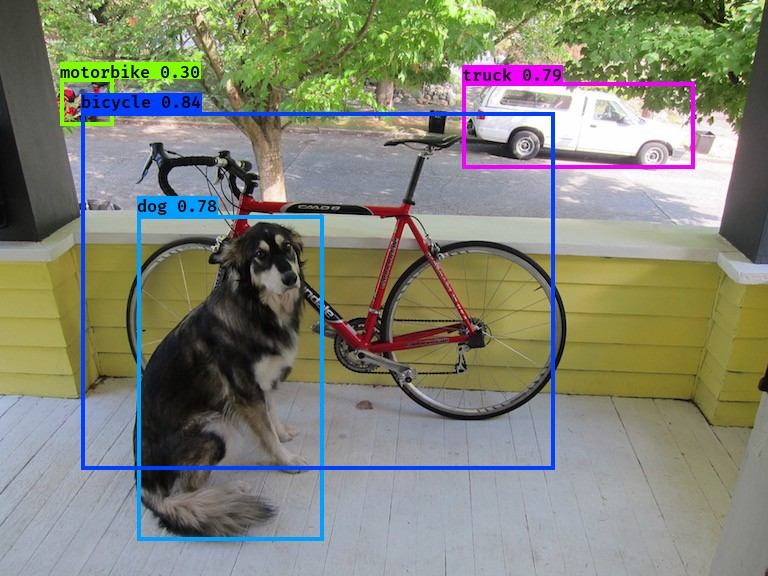
\includegraphics[width=0.5\linewidth]{images/dog}
		\caption{Sample of YOLOv2 detection working on an image on my machine.}
		\label{fig:dog}
	\end{figure}
	
	\begin{wrapfigure}{O}{0pt}
		\centering
		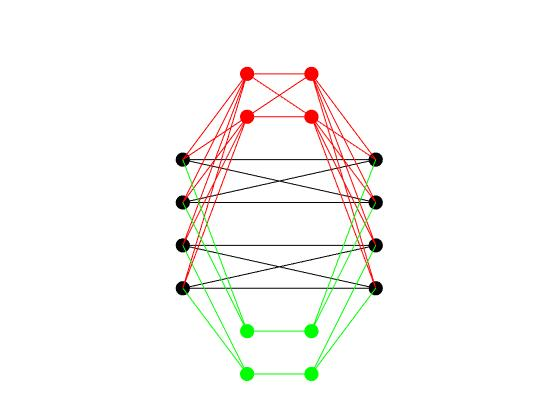
\includegraphics[width=0.5\textwidth]{HNN}
		\caption{Sample of proposed hierarchical layers.}
		\label{fig:hnn}
	\end{wrapfigure}
	
	
	\section{Methodology}
	\subsection{Re-training: In Process}
	After performing background research on image detection, network compression, and working with the Darve Group to understand previous work, the next step is to re-train the YOLOv2 network on the KITTI dataset. The algorithm currently runs on the images (see Figure \ref{fig:kitti_test}), but performance has not yet been evaluated on how the algorithm performs on the dev and test sets. Prior to retraining the network, the KITTI labels needed to be converted to the format expected by the yad2k model, so I wrote a conversion script that saves the data to \texttt{.npz} file. Since the training set is so large, I need to edit the retrain function of the model to read the files from disc, rather than expected them to be stored in a single array in memory. Once the model has been retrained on the KITTI dataset it will be ready be pruned. To speed training time during this and future steps, I'm currently learning how to run jobs on the Stanford Sherlock cluster.
	
	\begin{figure}
		\centering
		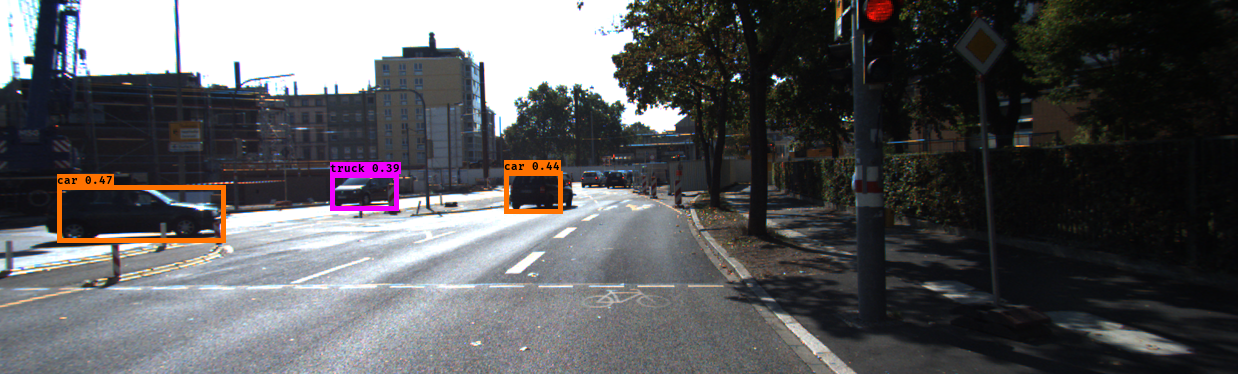
\includegraphics[width=\linewidth]{images/kitti_test}
		\caption{Example of un-refined YOLOv2 algorithm working on an image from the KITTI dataset. Currently running with labels from the MS COCO dataset.}
		\label{fig:kitti_test}
	\end{figure}
	
	\subsection{Pruning: Next Step}
	After the model is retained on the KITTI data set I will begin pruning the weights of the network by iteratively nullifying the lowest weights and retraining the entire network on the KITTI images. The weights of the network will be saved at each pruning iteration for subsequent analysis. We expect to find a threshold where any subsequent pruning results in dramatic decreases in both training and test set errors. By analyzing the weights at the pruned configuration versus the initial configuration we hope to gain some insight about what weights are important and what they mean in terms of the input and output. 
	
	\subsection{Exploring new topologies: Ambitious Goal}
	If the pruning steps don't take too long, I also plan to explore the use of hierarchical layers such as those shown in Figure \ref{fig:hnn}. The Darve Group has also shown some preliminary results that these type of layers may provide promising  behavior since they preserve the global connectivity of fully connected layers but with a significantly reduced number of edges. The authors of YOLO decided to remove the fully connected layers at the end of YOLO (v1) when implementing YOLOv2. This resulted in a slight drop in mAP, but an increase in recall. I plan to re-implement fully-connected layers at the end of YOLOv2, analyze performance, and then explore using hierarchical layers and analyze the difference in performance. 
	
	\section*{Code}
	My code is located at \url{https://github.com/bjack205/PrunedYOLO.git}. I have mostly focused on understanding the code I will be interfacing with, such as the KITTI dataset and the yad2k model, so haven't written very much yet.
	
	\printbibliography
	
	
	
	
	
\end{document}